\section{Primera sección}

% Citar una referencia
Esto es una referencia bibliográfica \cite{bibex}. Se recomienda leer ``The Not So Short Introduction to \LaTeX'' \cite{Oetiker2007} (existen versiones más modernas).


\subsection{Ecuaciones y fórmulas}

Gracias a la ecuación de Euler ($e^{ \pm i\theta } = \cos \theta \pm i\sin \theta$) podemos ver la relación entre varias de las constantes matemáticas más importantes:
\[
    e^{i\pi} + 1 = 0.
\]


% Fórmula numerada
Si una ecuación se va a referenciar es necesario numerarla:
\begin{eqnarray}
\label{eq:schemeP}
 \Phi (k)=\dfrac{2}{|R(k)|(|R(k)|-1)} \underset{i,j \in R(k)}{\sum} a_{ij}.
\end{eqnarray}
Posteriormente se hace referencia a la ecuación a través de su etiqueta (label). Por ejemplo, la anterior ecuación \eqref{eq:schemeP}.



Problema de optimización:
\begin{equation}\label{eq:LP1}
\begin{array}{cl}
  \displaystyle \begin{array}{c}\mathrm{minimizar} \\ \mathbf{t} \in \mathbb{R}^{n}, \  \mathbf{p} \in \mathbb{R}^{m} \end{array} & \hspace{-0.2cm} \begin{array}{c} \mathbf{1}^{\transpuesta}\mathbf{t} \\ \mbox{} \end{array}  \\
  & \vspace{-0.4cm} \\ % línea (fila) en blanco, pero la hacemos estrecha con el comando vspace
  \mbox{sujeto a} & -\mathbf{t} \preceq  \mathbf{V}\mathbf{p} - \mathbf{x}  \preceq  \mathbf{t},\\
 \end{array}
\end{equation}




\subsection{Tablas y figuras}

% Insertar una tabla
\begin{table}
  \centering
  \caption{Título de la tabla.}
  \label{tab:una_tabla}

\begin{footnotesize}
\renewcommand{\arraystretch}{1.5} % Para cambiar la separación entre filas (1 por defecto)
\begin{tabular}{ccccccccccc}
  \hline
   & Subs. & Students & A & PE & WA & RE & CTE & IF & TLE & All\\
  \hline
Ex. 1 & 104 & 44 & 1.27    &   0       &   0.55    &   0.23    &   0.20    &   0.11    &   0     & 2.36  \\
Ex. 2 & 118 & 37 & 0.92    &   0       &   0.92    &   0.27    &   0.49    &   0.59    &   0     & 3.19  \\
Ex. 3 & 100 & 28 & 1.21    &   0.39    &   1.18    &   0.54    &   0.14    &   0.07    &   0.04  & 3.57  \\
Ex. 4 & 78  & 25 & 1.08    &   0.84    &   0.52    &   0.40    &   0.24    &   0.04    &   0     & 3.12  \\
Ex. 5 & 116 & 31 & 1.48    &   0.10    &   0.77    &   0.32    &   0.42    &   0.19    &   0.45  & 3.74  \\
Ex. 6 & 213 & 32 & 1.06    &   0.34    &   3.81    &   0.56    &   0.69    &   0.06    &   0.13  & 6.66  \\
Ex. 7 & 116 & 34 & 1.35    &   0.38    &   0.38    &   0.68    &   0.62    &   0       &   0     & 3.41  \\
  \hline
Average & 120.7 & 33 & 1.20 &  0.26 &  1.14 &  0.42 &  0.40 &  0.16 &  0.08 & 3.66 \\
  \hline
 \end{tabular}
\end{footnotesize}

\end{table}









\begin{sidewaystable}
  \centering
  \caption{Tabla rotada. Factor groupings for the Mooshak questionnaire.}\label{tab:factor_analysis}

\renewcommand{\arraystretch}{1.1}
\begin{scriptsize}
 \begin{tabular}{clcc}
   \hline
   Factor & \textbf{Interpretation} / Items$^{*}$ (loadings)  & Median & Mode \\
   \hline
   \hline
    1 & \multicolumn{3}{l}{\textbf{Students' perception of Mooshak towards its helpfulness in learning} } \\
   \hline
    (21.17\%) & m10. Mooshak has forced me to implement programs more carefully $(0.849)$ & 4 & 4 \\
    $\alpha$ = 0.922 & m6.  Mooshak has helped me improve as a programmer $(0.819)$ & 3 & 4 \\
     & m5.  Mooshak has made me more aware of the need to write correct code $(0.781)$ & 3 & 3\\
     & m1. Mooshak has forced me to program more responsibly $(0.713)$ & 3 & 3 \\
     & m15. The specifications regarding the exercises used with Mooshak are adequate $(0.687)$ & 3 & 3 \\
     & m18. Mooshak helps to measure my current programming skills $(0.680)$ & 2.5 & 3 \\
   \hline
%   \multicolumn{4}{c}{} \vspace{-0.2cm}\\
%   \hline
    2 & \multicolumn{3}{l}{\textbf{Disposition towards using Mooshak} } \\
   \hline
    (17.93\%) & m24. I would be willing to participate in a programming contest using Mooshak, with similar exercises to the ones & 2 & 1 \\
    $\alpha$ = 0.897 & seen throughout the course $(0.807)$ & & \\
    & m13. Using Moohak in the final exams is a good idea $(0.748)$ & 2 & 1 \\
    & m14. I would like to use Mooshak or a similar tool in the future $(0.734)$ & 3 & 1 \\
    & m17. Knowing Mooshak can motivate me to take part in a programming contest $(0.655)$ & 2 & 1\\
    & m9. It would have been useful to use Mooshak from the first programming course $(0.527)$ & 2.5 & 1\\
     & m16. Using Mooshak in the course has been interesting $(0.522)$ & 3 & 4 \\
   \hline
%   \multicolumn{4}{c}{} \vspace{-0.2cm}\\
%   \hline
    3 & \multicolumn{3}{l}{\textbf{Effect of Mooshak's feedback in the tool's usefulness} } \\
   \hline
    (14.84\%) & m12. Mooshak's feedback is adequate $(0.832)$ & 2 & 1\\
    $\alpha$ = 0.836 & m3. Using Mooshak has increased my workload considerably $(0.693)$ & 4 & 4 \\
     & m7.  If Mooshak does not accept my code I feel motivated to find and fix the errors $(0.691)$ & 2 & 3 \\
     & m8.  In general, using Mooshak has been a good idea $(0.666)$ & 3 & 4 \\
   \hline
%   \multicolumn{4}{c}{} \vspace{-0.2cm}\\
%   \hline
    4 & \multicolumn{3}{l}{\textbf{Mooshak's effect on persistence} } \\
   \hline
    (11.20\%) & m23. When Mooshak does not accept my code I get discouraged and I abandon the exercise $(0.848)$ & 3 & 3 \\
    $\alpha$ = 0.705 & m22. Mooshak has been a waste of time $(0.597)$ & 2 & 2 \\
    & m25. Once a program has passed Mooshak's tests, I rewrite it in order to enhance it $(0.559)$ & 2 & 2 \\
   \hline
%   \multicolumn{4}{c}{} \vspace{-0.2cm}\\
%   \hline
   5 & \multicolumn{3}{l}{\textbf{Students' perception of Mooshak's features} } \\
   \hline
    (10.87\%) & m20. Even if it is not related to the grade, I feel satisfied if I am one of the first students to complete an exercise $(0.729)$ & 2 & 2\\
   $\alpha$ = 0.742  & m19. I value the fact that a tool like Mooshak returns feedback in real time about the correction of my programs $(0.650)$ & 3.5 & 4 \\
   \hline
%   \multicolumn{4}{c}{} \vspace{-0.2cm}\\
%   \hline
\multicolumn{4}{l}{\scriptsize $^{*}$Measured on a 5-point Likert scale (1: strongly disagree; 2: disagree; 3: neutral; 4: agree; 5: strongly agree).}
  \end{tabular}
\end{scriptsize}
\end{sidewaystable}



\begin{table}
  \centering

\begin{small}
\begin{tabular}{|l|l|l|l|}\hline
  \multirow{10}{*}{numeric literals} & \multirow{5}{*}{integers} & in decimal & \verb|8743| \\ \cline{3-4}
  & & \multirow{2}{*}{in octal} & \verb|0o7464| \\ \cline{4-4}
  & & & \verb|0O103| \\ \cline{3-4}
  & & \multirow{2}{*}{in hexadecimal} & \verb|0x5A0FF| \\ \cline{4-4}
  & & & \verb|0xE0F2| \\ \cline{2-4}
  & \multirow{5}{*}{fractionals} & \multirow{5}{*}{in decimal} & \verb|140.58| \\ \cline{4-4}
  & & & \verb|8.04e7| \\ \cline{4-4}
  & & & \verb|0.347E+12| \\ \cline{4-4}
  & & & \verb|5.47E-12| \\ \cline{4-4}
  & & & \verb|47e22| \\ \cline{1-4}
  \multicolumn{3}{|l|}{\multirow{3}{*}{char literals}} & \verb|'H'| \\ \cline{4-4}
  \multicolumn{3}{|l|}{} & \verb|'\n'| \\ \cline{4-4}          %% here
  \multicolumn{3}{|l|}{} & \verb|'\x65'| \\ \cline{1-4}        %% here
  \multicolumn{3}{|l|}{\multirow{2}{*}{string literals}} & \verb|"bom dia"| \\ \cline{4-4}
  \multicolumn{3}{|l|}{} & \verb|"ouro preto\nmg"| \\ \cline{1-4}          %% here
\end{tabular}
\end{small}

  \caption{Tabla con ``multicolumnas'' y ``multifilas''.}\label{tab:tablacompleja}
\end{table}





% Insertar una figura
\begin{figure}
  \centering
  \includegraphics[width=0.75\textwidth,clip=true]{\logoUniversidad}
  \caption{Logo de la Universidad.}
  \label{fig:logo_universidad}
\end{figure}

% Referenciar una etiqueta (label)
Las tablas y figuras deben presentarse en el texto, referenciadas y numeradas. La descripción de una figura debe ir posicionada debajo de la misma. Las descripciones de tablas pueden aparecer encima o debajo de las mismas (pero de forma consistente en todo el documento).

En las tablas se recomienda evitar líneas verticales y usar pocas horizontales. 

La figura~\ref{fig:logo_universidad} se utiliza en la portada. \LaTeX ubica automáticamente las tablas y figuras. Para ello emplea reglas basadas en la experiencia de profesionales de la edición de textos. Podemos forzar su ubicación, pero en general es recomendable usar la ubicación sugerida por el sistema \LaTeX. Usad gráficos vectoriales siempre que podáis.





\begin{figure}
   \centering

  \begin{minipage}{0.45\textwidth}
   \centering

     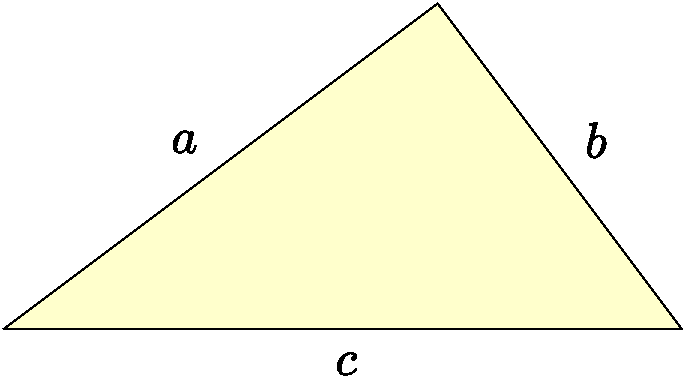
\includegraphics[clip=true,width=\textwidth]{triangulo_grande_bb.pdf}\\

    \footnotesize (a)
  \end{minipage}
  \hfill
  \begin{minipage}{0.45\textwidth}
   \centering
     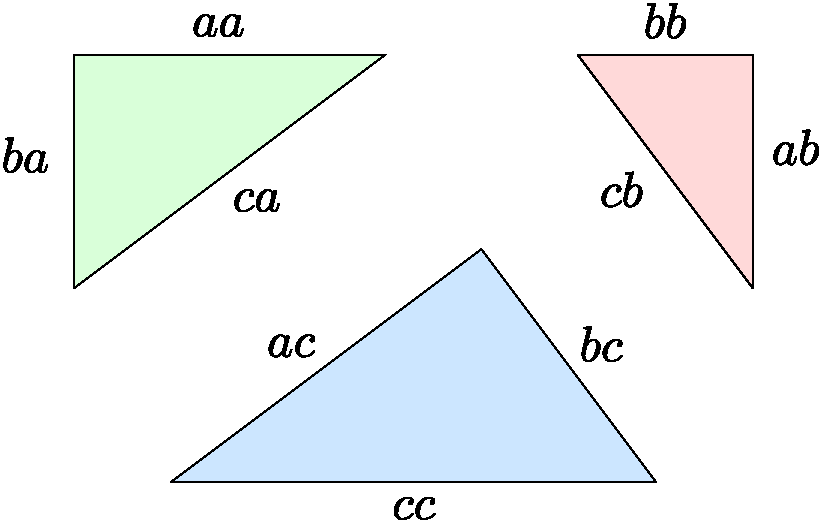
\includegraphics[clip=true,width=\textwidth]{triangulos_separados_bb.pdf}\\

   \footnotesize (b)
  \end{minipage}

    \bigskip

    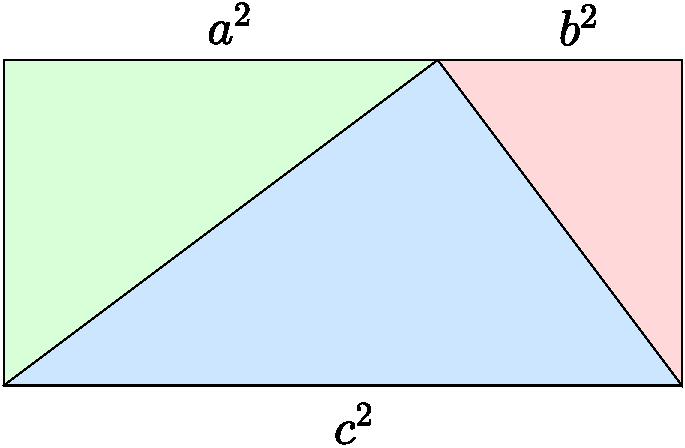
\includegraphics[clip=true,width=0.5\textwidth]{triangulos_unidos_bb.pdf}\\
    \footnotesize (c)

  \caption{Ejemplo con varias figuras. Demostración visual del teorema de Pitágoras. En (a) tenemos un triángulo rectángulo con hipotenusa $c$ y catetos $a$ y $b$. En (b) se muestra tres copias escaladas del mismo triángulo. El verde se ha escalado por $a$, el rojo/rosa por $b$, y el azul por $c$. En (c) se juntan los triángulos de (b) para formar un rectángulo cuya base es $c^{2}$, pero también $a^{2} + b^{2}$. Por tanto, $a^{2} + b^{2} = c^{2}$.}\label{fig:teoremapitagoras}
\end{figure}





\section{Segunda sección}

% Nueva página
Normalmente no tendremos que insertar saltos de página, salvo para forzar que los capítulos empiecen en páginas impares, con \begin{verbatim}\blankpage\end{verbatim} En cualquier caso, podemos introducir un salto de página con el comando \begin{verbatim}\newpage\end{verbatim}.

\newpage
% También con \pagebreak



\subsection{Código}


\begin{mypython}[float={!t},caption={Titulo del algoritmo/código.},label={alg:etiqueta}]
def sum_list_limits_1(a, lower, upper):
    if lower > upper:
        return 0
    else:
        return a[upper] + sum_list_limits_1(a, lower, upper - 1)
\end{mypython}
El código~\ref{alg:etiqueta} es un ejemplo en Python.



\begin{algorithm}
\begin{algorithmic}[1]
\STATE $\forall i \in V$, \ let $i$ be an isolated community
\STATE $o=permutation(V)$
\FOR{$k \ \in \ o$}
\STATE search in $A$ all the neighbours of $k$, $j$
\STATE $\forall j$, calculate $\Delta Q_k(j)$ in matrix $\mathcal{M}$
\STATE $j^*=\{ \ j \ | \ \Delta Q_k(j^*)=\max_j\{Q_k(j)\} \ \}$
\IF{$\Delta Q_k(j^*)>0$}
\STATE{Move node $k$ to $j^*$ 's community}
\ELSE
\STATE{$k$ remains in its community}
\ENDIF
\ENDFOR
\end{algorithmic}\caption{\textit{Additional Louvain} \textbf{input}=$\left(A, \ \mathcal{M}\right)$ \textbf{output}=$P$}
\label{alg:AdditionalLouvain}
\end{algorithm}
En el algoritmo~\ref{alg:AdditionalLouvain} aparece un ejemplo en pseudocódigo.